% Procediamo ora secondo la strategia Top-down raffinando le definizioni delle entità e aggiungendo ulteriori relazioni.
% \subsubsection{Personaggio}
% Sappiamo che il personaggio ha parecchie caratteristiche e valori che lo contraddistinguono, possiamo suddividerle in 4 gruppi:
% Posizione, Fisico, Statistiche e Statistiche totali
%
% \begin{figure}[H]
% \centering
% 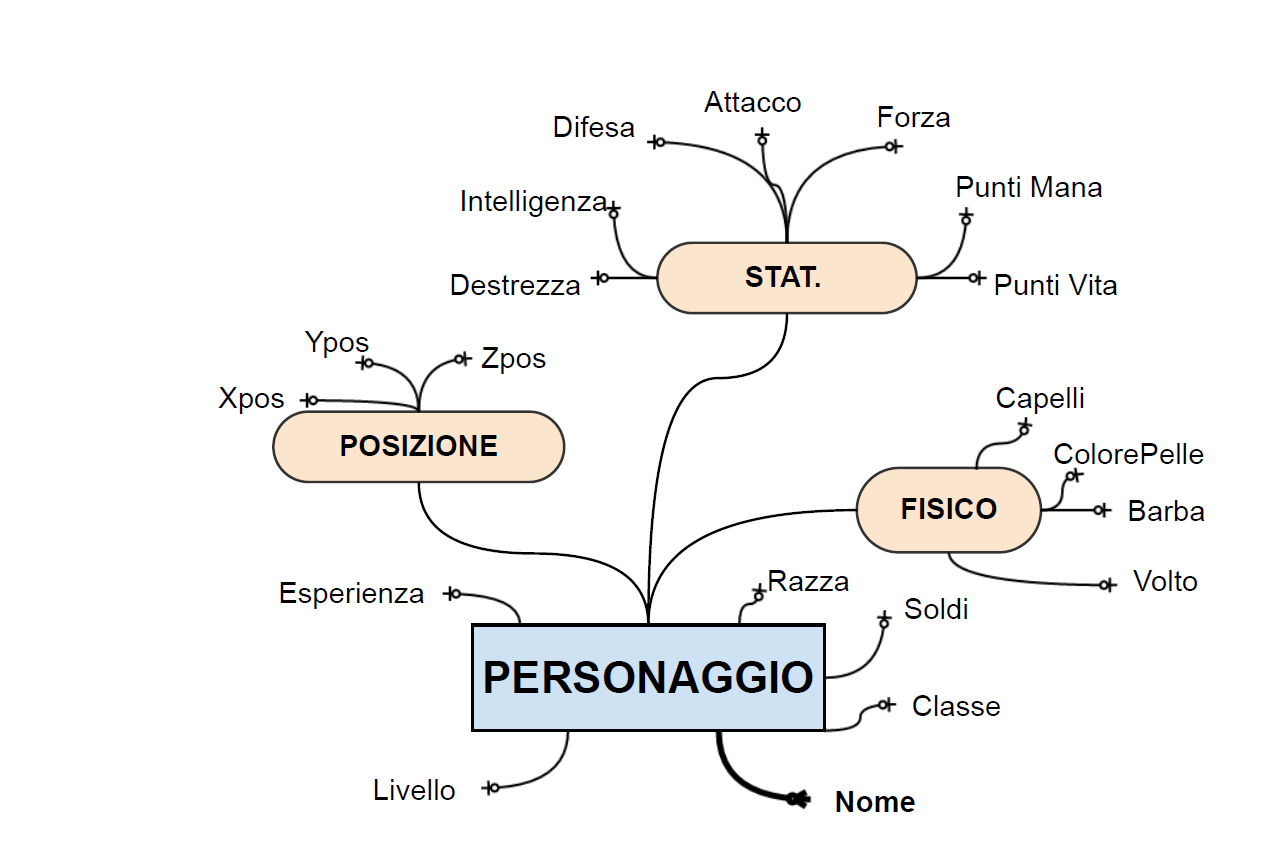
\includegraphics[width=0.7\linewidth]{./immagini/personaggiodef.png}
% \end{figure}
%
% \newpage
%
%
% \subsubsection{NPC}
% Gli npc sono divisi principalmente in ostili e amichevoli, questo ne determina fortemente la funzione all'interno del gioco, le relazioni con le altre entità nonchè i dati stessi che essi utilizzano, è quindi necessaria una Generalizzazione che i suddivida di conseguenza
%
% \begin{figure}[H]
% \centering
% 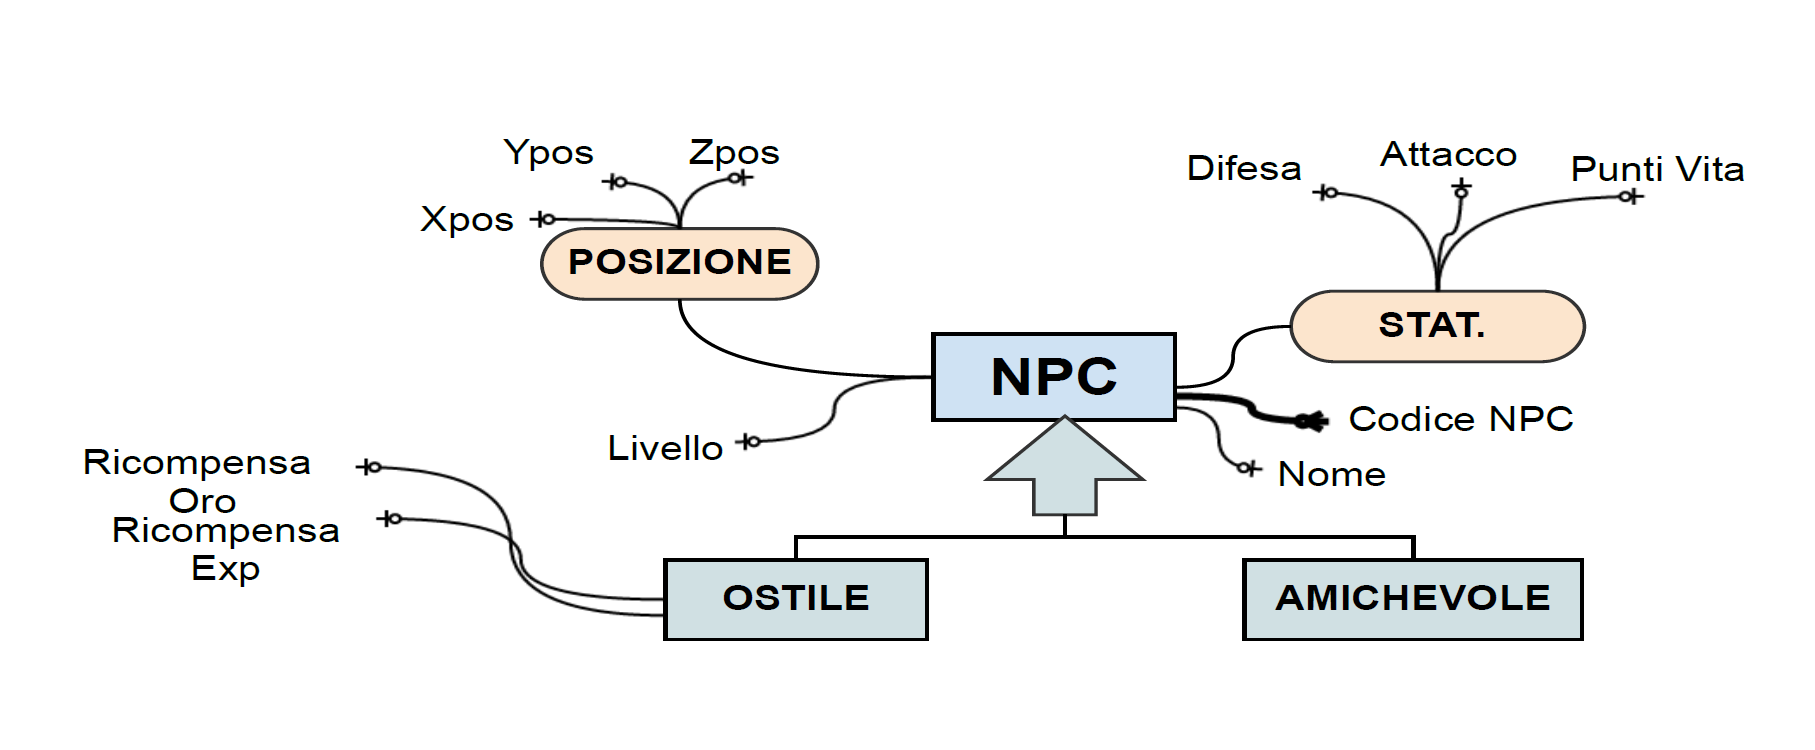
\includegraphics[width=0.7\linewidth]{./immagini/npcdef.png}
% \end{figure}
%
%
% \subsubsection{Oggetto}
% Per gli oggetti sappiamo che alcuni di essi possono essere equipaggiati, consumati dal personeggio oppure essere oggetti missione, questo fatto oltre a comportare una Generalizzazione implica la necessità di una relazione di equipaggiamento, una di consumo e una di stock per descrivere la proprietà di un OGGETTO da parte di un PERSONAGGIO
%
% \begin{figure}[H]
% \centering
% 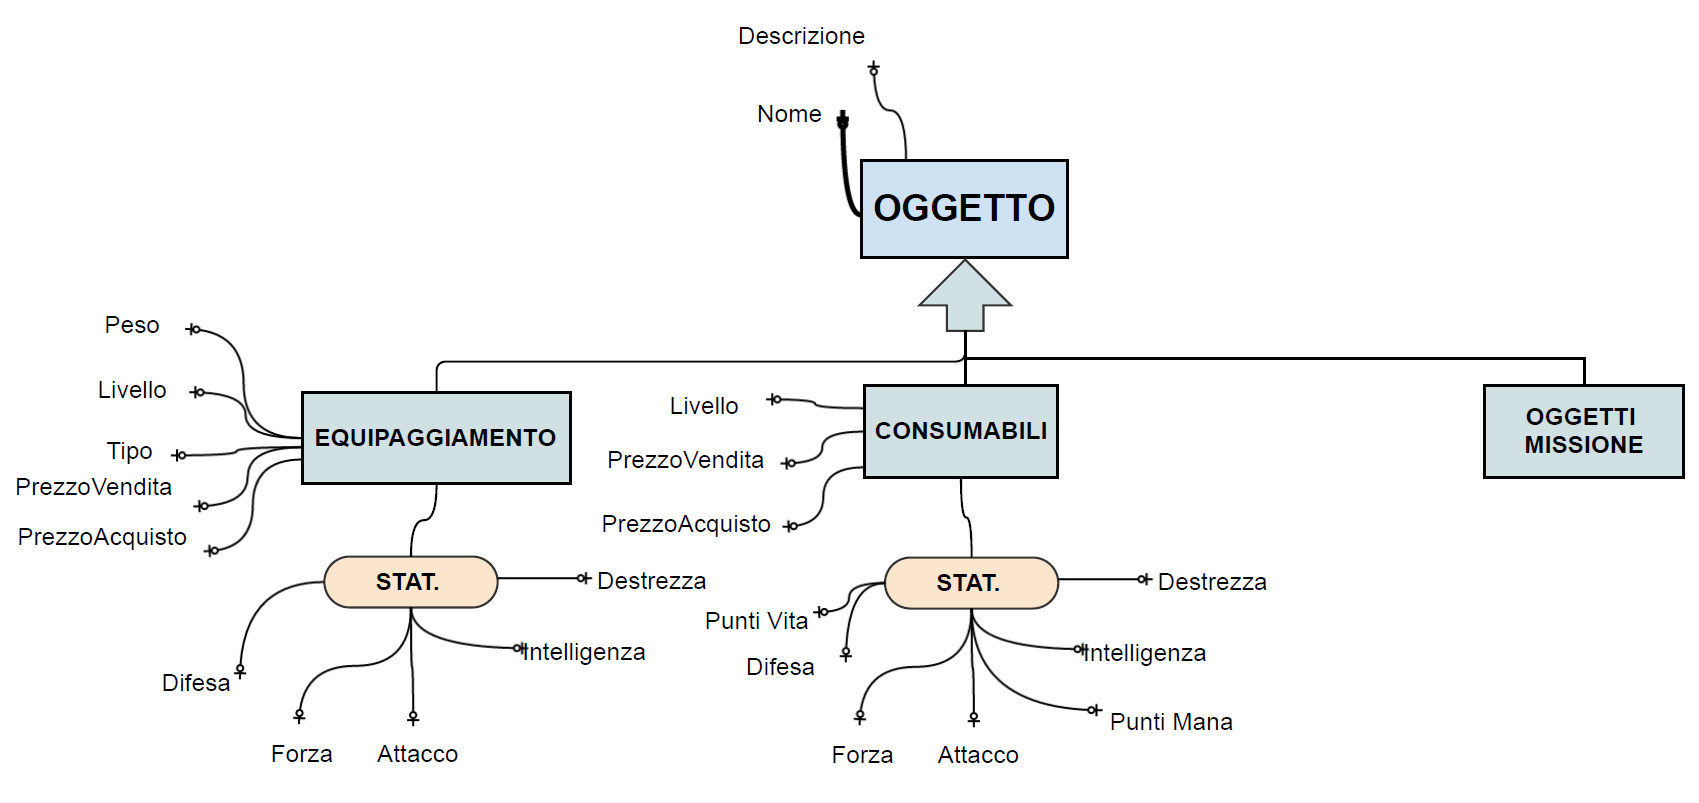
\includegraphics[width=0.7\linewidth]{./immagini/oggettodef.png}
% \end{figure}
%
%  \newpage
%
% \subsubsection{Abilità}
% Dalle interviste sappiamo che le abilità hanno svariati attributi che sono poi i valori da sommare alle statistiche dei personaggi che imparano le abilità, hanno anche un costo e un livello massimo.
%
% \begin{figure}[H]
% \centering
% 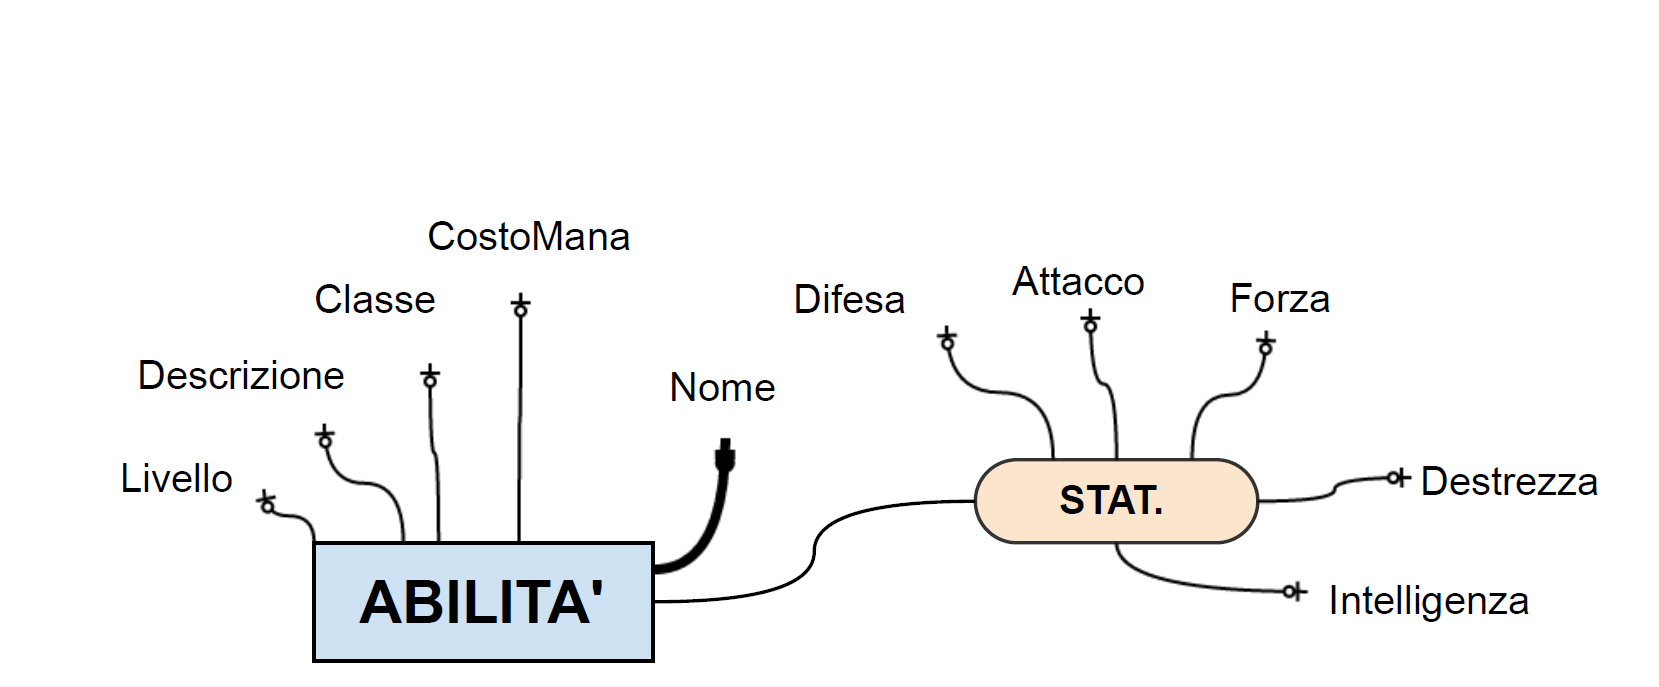
\includegraphics[width=0.7\linewidth]{./immagini/ABILITADEF.png}
% \end{figure}
%
% \subsubsection{Transazione}
% Le transazioni saranno necessarie solo per tenere traccia degli acquisti della sessione, esse avranno un SOGGETTO e un OGGETTO intesi come "chi vende a chi compra"
%
% \begin{figure}[H]
% \centering
% 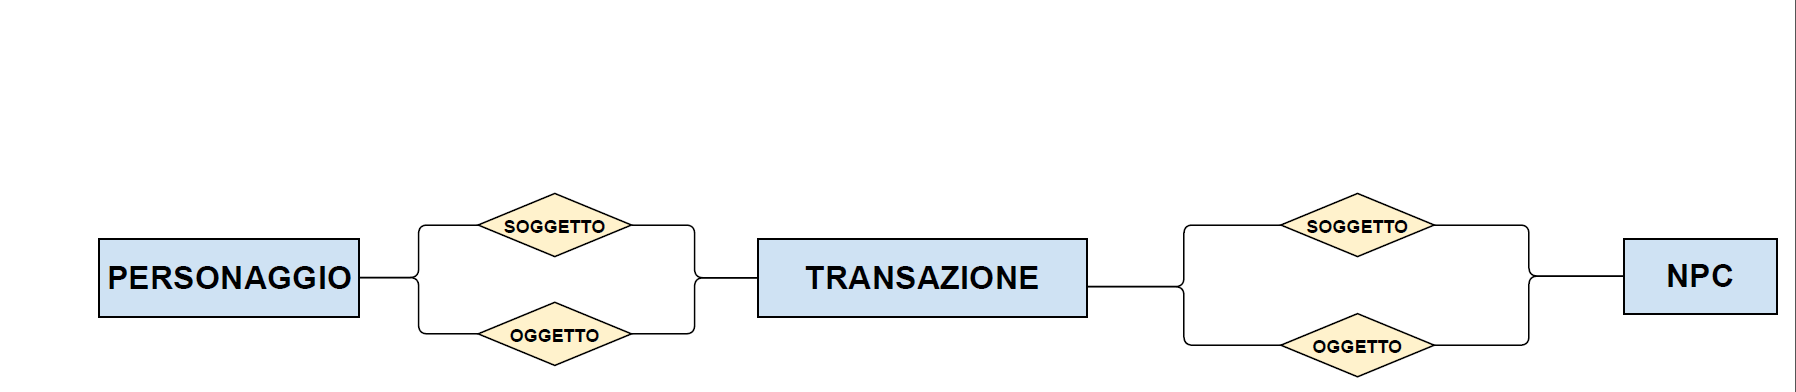
\includegraphics[width=0.7\linewidth]{./immagini/TRANSAZ.png}
% \end{figure}
% AMBIGUITA
%
% \subsubsection{Utente}
% L'utente è la persona vera e propria che si logga per giocare con uno dei suoi personaggi, puo fare acquisti nello Store con una delle sue carte di credito, eliminare o creare personaggi e modificare i suoi dati di fatturazione.
%
%
% \begin{figure}[H]
% \centering
% 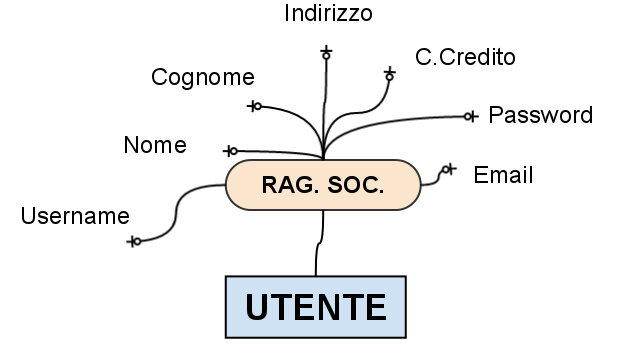
\includegraphics[width=0.7\linewidth]{./immagini/untentedef.png}
% \end{figure}
%
% \subsubsection{Prodotto}
% I PRODOTTI nel nostro gioco sono principalmente 3, cioè le SOTTOSCRIZIONI, I PACCHETTI OGGETTI che permettono di acquistare un gruppo di oggetti Elencati e le ESPANSIONI del Gioco che permettono di raggiungere un livello massimo piu alto.
%
% \begin{figure}[H]
% \centering
% 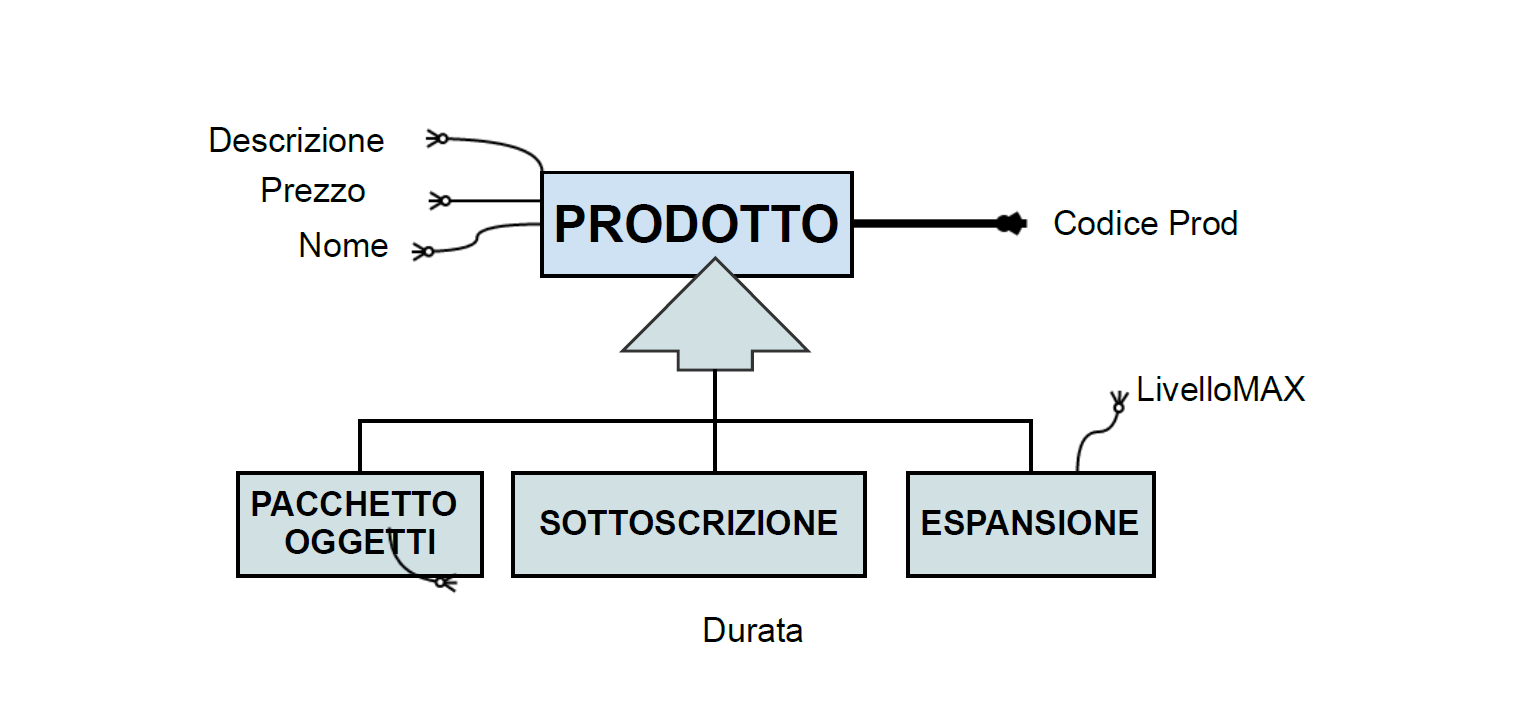
\includegraphics[width=0.7\linewidth]{./immagini/prodottodef.png}
% \end{figure}
%
% \newpage
